\documentclass{subfiles}

\begin{document}
    \marginnote{\textbf{\textit{VL 2}}\\27.04.2023, 10:00}

    \subsubsection*{Gaußsches Wellenpaket}
        Als fundamentale Funktion eines Wellenpaketes zählt das sogenannte \textit{Gaußsche Wellenpaket}. Es wird beschrieben durch die Funktion 
        \[\psi(k) = A\cdot\exp(\frac{-(k - k_0)^2}{4\cdot\pi^2}),\quad \psi\in\Abb{\R^3}{\R^3},\]
        wobei $4\pi^2$ mit der \enquote{Breite} korreliert und $k_0$ der \emph{mittlere Wellenvektor} ist. Die Funktion hat die Form
        \begin{figure}[H]
            \centering
            \begin{tikzpicture}
                \begin{axis}
                    \addplot[domain=-10:10,smooth,samples=100]{exp(-(x-1)^2/(4*3.141592))};
                \end{axis}
            \end{tikzpicture}
            \caption{Die Gaußkurve für $A=1$, $k_0=1$ in $\R$.}
        \end{figure}
        Das Ergebnis der Fourier-Summation angewendet auf die Gaußfunktion ergibt 
        \[\abs{\psi(t,r(t))}^2 = \frac{1}{\sqrt{2\cdot\pi}\cdot w(t)}^{\frac{3}{2}}\cdot\exp(-\frac{(r(t)-v\cdot t)^2}{2\cdot w(t)^2})\]
        mit der Definition $v:=\hbar\cdot k/m = \Dvat{t}{\omega(k_0 + t\cdot h)}{0} = d\omega(k_0)(h)$ und $w(t) := \sqrt{w(0)^2 + ((\hbar\cdot t)/(2\cdot w(0)\cdot m))}$ mit dem Startwert $w(0) = 1/(2\cdot\sigma)$. 

        \begin{Aufgabe}
            \nr{} Man spricht bei Fourier-Summationen vom \emph{Raumwechsel}. Was ist damit gemeint? Welche Räume haben wir hier verwendet?

            \nr{} Zeichne das Ergebnis einmal graphisch für dieselben Parameter wie oben. Was fällt dir auf?

            \nr{} Welches $h\in\R^3$ ist bei der Ableitung $d\omega(k_0)(h)$ gemeint?
        \end{Aufgabe}
        
        \begin{figure}[H]
            \centering
            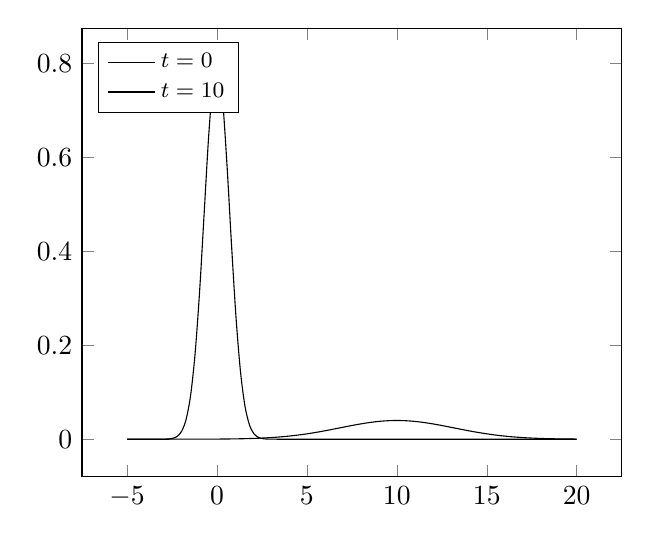
\begin{tikzpicture}
                \pgfplotsset{legend style={font=\footnotesize}}
                \begin{axis}[legend cell align=left,legend pos=north west]
                    \addplot[domain=-5:20,smooth,samples=100]{(1/(sqrt(2*3.141592) * sqrt((1/2)^2 + (1*0/(2*(1/2)*1))^2)))*exp(-(x-0)^2/(2 * sqrt((1/2)^2 + (1*0/(2*(1/2)*1))^2)))};
                    \addlegendentry{$t=0$}
                    \addplot[domain=-5:20,smooth,samples=100]{(1/(sqrt(2*3.141592) * sqrt((1/2)^2 + (1*10/(2*(1/2)*1))^2)))*exp(-(x-10)^2/(2 * sqrt((1/2)^2 + (1*10/(2*(1/2)*1))^2)))};
                    \addlegendentry{$t=10$};
                \end{axis}
            \end{tikzpicture}
            \caption{Die Forier-Summierte Gaußkurve für $A=1$, $k_0=1$ in $\R$ zum Zeitpunkt $t=0$ und $t=10$}
        \end{figure}

        \subsubsection*{Zusammenfassung}
            \begin{itemize}[label=$\to$]
                \item Das Wellenpaket bewegt sich mit der Aufenthalserwartung 
                \[\langle r(t)\rangle = \lint{\fdef{r\cdot\abs{\psi(t,r)}}{r\in\R^3}}{r}{}.\]
                \item Das Wellenpaket im Ortsraum ist ebenfalls eine Gaußfunktion mit Peakbreite $w(t)$ und Startwert $w(0) = 1/(2\cdot\sigma)$. 
                \item Das Wellenpaket erfährt Dispersion für $t>0$ durch die Funktionsdefinition $w$:
                \item Für $t>> w(0)^2\cdot m/\hbar$ ist $w(t) \approx \hbar\cdot t/(2\cdot w(0)\cdot m)$ linear von $t$ abhängig. Für lange $t$ ist die Dispersion also linear (und nicht proportional zu $\sqrt{t}$). 
                \item Für die Mittelung $\langle r(t)\rangle$ folgt 
                \[\Delta r^2 := \langle r(t_1) - \langle r(t_0)\rangle\rangle = \lint{\fdef{(r-\langle r\rangle)\cdot\abs{\psi(t,r)}}{r\in\R^3}}{r}{} = w(t)^2.\]
            \end{itemize}
            \begin{Aufgabe}
                \nr{1} Berechne die Integrale $\lint{x\cdot\exp(-x^2)}{x}{}$, $\lint{x\cdot\exp(-(x-x_0)^2)}{x}{}$ und $\lint{(x-x_0)\cdot\exp(-(x-x_0)^2)}{x}{}$ für $x_0\in\R$ auf $(\R,\sigma(\R),\lambda)$. Wie ist die Struktur?
    
                \nr{} Rechne die Dispersion des Wellenpaketes für $t>0$ gemäß $w$ nach und zeige $w(t)^2>w(0)$. 
            \end{Aufgabe}

    \subsection{Die Heisenbergsche Unschärferelation (I)}
        Zunächst bemerken wir die Eigenschaft der \emph{Normerhaltung} gemäß des \href{https://de.wikipedia.org/wiki/Satz_von_Parseval}{\emph{Satzes von Parseval}} der Fourier-Summation. Es gilt 
        \[\lint{\abs{\psi(t,r)}^2}{r}{} = \lint{\frac{\abs{\tilde\psi(k)}^2}{(2\cdot\pi)^3}}{k}{} = \lint{\frac{\abs{\tilde\psi(p)}^2}{(2\cdot\pi\cdot\hbar)^3}}{p}{}\]
        und für die Mittelung
        \[\langle p\rangle = \lint{\frac{p\cdot\abs{\tilde\psi(p)}^2}{(2\cdot\pi\cdot\hbar)^3}}{p}{} := \lint{\frac{p\cdot\exp(-\frac{(p-p_0)^2}{4\cdot\hbar^2\cdot\sigma^2})}{(2\cdot\pi\cdot\hbar)^3}}{p}{} \stackrel{\refnr{1}}{=} p_0 = \hbar\cdot k_0.\]
        Die mittlere Schwankung, also physikalisch die Genauigkeit des Impulses im Impulsraum, ergibt sich zu
        \[\Delta p^2 = \langle (p-\langle p\rangle^2)^2\rangle = \hbar^2\cdot\sigma^2,\]
        wobei unter Verwendung von $\Delta r^2 = w(t)^2$ folgt
        \[\Delta r^2 = w(t)^2\geq \nbra{\frac{1}{2\cdot\sigma}}^2 = \frac{1}{4\cdot\sigma^2},\]
        sodaß mit beiden Gleichungen unter Produktbildung und Wurzelzug eine Ausdrucksweise der Unschärferelation, konkret jene von Heisenberg, folgt:
        \[\Delta r \cdot\Delta p \geq \frac{\hbar}{2}.\]
        \begin{Aufgabe}
            \nr{} Lässt sich die Wellenfunktion direkt experimentell bestimmen? Recherchiere die \href{https://de.wikipedia.org/wiki/Quantentomographie}{\emph{Quanten-Zustands-Tomographie}}.
        \end{Aufgabe}

        \subsubsection*{Physikalische Bedeutung}
            Aus der Unschärferelation folgen folgende physikalische Konsequenzen:
            \begin{itemize}[label=$\to$]
                \item Unmittelbar ist ablesbar, daß bei genauerer Ortsbestimmung die Impulsgenauigkeit abnimmt. 
                \item Für $\Delta p\to 0$ (Fall ebene Welle) ist $\Delta r \to \infty$. 
                \item Der Phasenraum ist infolge der Unschärferelation quantisiert in Einheiten von $\hbar$.
            \end{itemize}


\end{document}